\documentclass[a4paper,11pt]{scrartcl}
\usepackage[T1]{fontenc}
\usepackage[utf8x]{inputenc}
\usepackage{graphicx}
\usepackage{xcolor}

% \usepackage{tgheros}
% \usepackage[defaultmono]{droidmono}

\usepackage{amsmath,amssymb,amsthm,textcomp}
\usepackage{enumerate}
\usepackage{multicol}
\usepackage{tikz}

\usepackage{menukeys}

\usepackage{geometry}
\geometry{total={210mm,297mm},
left=25mm,right=25mm,%
bindingoffset=0mm, top=20mm,bottom=30mm}

\linespread{1.2}

\newcommand{\linia}{\rule{\linewidth}{0.5pt}}

% my own titles
\makeatletter
\renewcommand{\maketitle}{
\begin{center}
\vspace{2ex}
{\huge \@title}
\vspace{1ex}
\\
\linia\\
\@author \hfill \@date
\vspace{4ex}
\end{center}
}
\makeatother
%%%

% custom footers and headers
\usepackage{fancyhdr}
\pagestyle{fancy}
\lhead{}
\chead{}
\rhead{}
\lfoot{\mytitle}
\cfoot{}
\rfoot{\thepage}
\renewcommand{\headrulewidth}{0pt}
\renewcommand{\footrulewidth}{0.5pt}

%

% code listing settings
\usepackage{listings}
\lstset{
    language=Python,
    basicstyle=\ttfamily\small,
    aboveskip={1.0\baselineskip},
    belowskip={1.0\baselineskip},
    columns=fixed,
    extendedchars=true,
    breaklines=true,
    tabsize=4,
    prebreak=\raisebox{0ex}[0ex][0ex]{\ensuremath{\hookleftarrow}},
    frame=lines,
    showtabs=false,
    showspaces=false,
    showstringspaces=false,
    keywordstyle=\color[rgb]{0.627,0.126,0.941},
    commentstyle=\color[rgb]{0.133,0.545,0.133},
    stringstyle=\color[rgb]{01,0,0},
    numbers=left,
    numberstyle=\small,
    stepnumber=1,
    numbersep=10pt,
    captionpos=t,
    escapeinside={\%*}{*)}
}

% Inline graphics
\usepackage{graphicx,calc}
\newlength\myheight
\newlength\mydepth
\settototalheight\myheight{Xygp}
\settodepth\mydepth{Xygp}
\setlength\fboxsep{0pt}
\newcommand*\inlinegraphics[1]{%
  \settototalheight\myheight{Xygp}%
  \settodepth\mydepth{Xygp}%
  \raisebox{-\mydepth}{\includegraphics[height=\myheight]{#1}}%
}

% Swift
\lstdefinelanguage{swift}
{
  morekeywords={
    func,if,then,else,for,in,while,do,switch,case,default,where,break,continue,fallthrough,return,
    typealias,struct,class,enum,protocol,var,func,let,get,set,willSet,didSet,inout,init,deinit,extension,
    subscript,prefix,operator,infix,postfix,precedence,associativity,left,right,none,convenience,dynamic,
    final,lazy,mutating,nonmutating,optional,override,required,static,unowned,safe,weak,internal,
    private,public,is,as,self,unsafe,dynamicType,true,false,nil,Type,Protocol,
  },
  morecomment=[l]{//}, % l is for line comment
  morecomment=[s]{/*}{*/}, % s is for start and end delimiter
  morestring=[b]" % defines that strings are enclosed in double quotes
}
\definecolor{keyword}{HTML}{BA2CA3}
\definecolor{string}{HTML}{D12F1B}
\definecolor{comment}{HTML}{008400}
\lstset{
  language=swift,
  basicstyle=\ttfamily,
  showstringspaces=false, % lets spaces in strings appear as real spaces
  columns=fixed,
  keepspaces=true,
  keywordstyle=\color{keyword},
  stringstyle=\color{string},
  commentstyle=\color{comment},
}
\lstset{language=Swift}

\begin{document}

\newcommand{\mytitle}{TP 2 - Adaptive User Interfaces}
\title{\mytitle}
\author{Adrien Humilière}
\date{21/02/2018}

\maketitle

\section*{Part 1}

\begin{itemize}
\item Open, build and run (\keys{\cmd+R}) the \textbf{Flashlight} project.
\item Observe the size of the simulator on the screen. Use the menu item \menu[,]{Window,Scale} to adjust the size of the simulator screen       .
\item This is a really basic application template. Use it to discover Xcode interface anatomy.
\item Use \keys{\cmd+\tab} and \keys{\cmd+.} to switch to the simulator and back; and to stop the app from Xcode.
\end{itemize}

\section*{Part 2}

\begin{itemize}
\item Open and run (\keys{\cmd+R}) the \textbf{WordCollage} project.
\item Using the Project Navigator (\keys{\cmd+1}), explore \textbf{Main.storyboard}.
\item Using the Show Document Outline control (\inlinegraphics{../assets/show-document-outline.png}) in the lower left corner of the canvas, ensure that the document outline is visible.
\item Double-click a Label in the collage to change its contents.
\item Run the app (\keys{\cmd+R}), and witness the change in the iOS Simulator.
\item Experiment with changing the content of the remaining labels to topics you care about.
\item Run the app (\keys{\cmd+R}), and witness the changes in the Simulator.
\end{itemize}

\section*{Part 3}

\begin{itemize}
\item Use the Project Navigator (\keys{\cmd+1}) to select Main.storyboard.
\item Run the app (\keys{\cmd+R}), and observe how the visual layout of the collage appears different in the iOS Simulator.
\item Using the Object Library (\keys{\Alt+\cmd+L}), place a new Label on the interface. Change the Label contents (e.g. "Learn to Code") and use the Attributes Inspector (\keys{\Alt+\cmd+4}) to change the font family, size and color (e.g. 51pt Avenir Next Ultra Light).
\item Use the Label handles to expand its size, and adjust the Label position.
\item Run the app (\keys{\cmd+R}), and observe how the Label position appears differently in the iOS Simulator.
\item Position constraints must be added to the Label to influence its position.
\item With the Label selected, use the Pin control to select a Vertical Space constraint relative to the View.
\begin{figure}[h]
	\begin{center}
   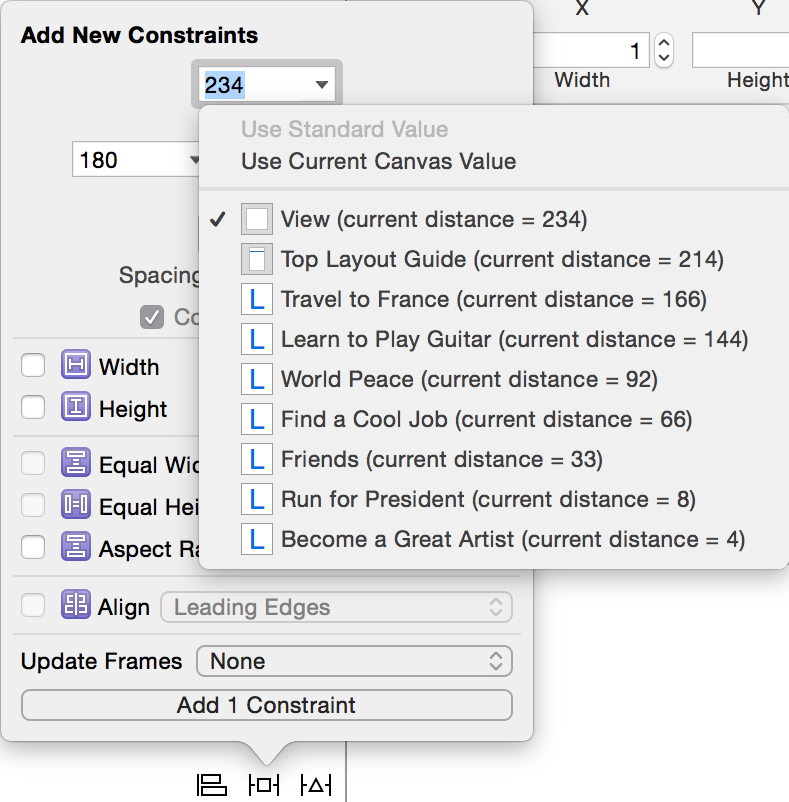
\includegraphics[width=200pt]{pin_constraint.png}
	\end{center}
\end{figure}
\item Interface Builder displays a vertical blue bar representing the Vertical Space constraint. Missing constraints result in Interface Builder displaying Auto Layout issues in orange.
\item With the Label selected, use the Align control to select a Center X Alignment constraint based on the current position of the Label.
\begin{figure}[h]
	\begin{center}
   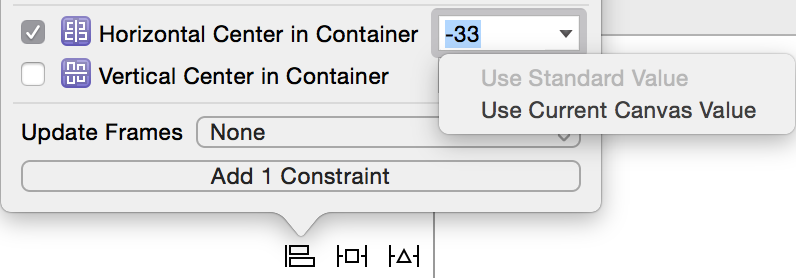
\includegraphics[width=200pt]{align_constraint.png}
	\end{center}
\end{figure}
\item Interface Builder displays another vertical blue bar representing the Center X Alignment constraint.
\item Using the Show Document Outline control (\inlinegraphics{../assets/show-document-outline.png}) in the lower left corner of the canvas, ensure that the document outline is visible.
\item Interface Builder displays one remaining Auto Layout issue in orange. Use the Issue Navigator (\keys{\cmd+4}) or the Document Outline disclosure arrow (\inlinegraphics{../assets/disclosure_arrow.png}) to observe the details of the remaining Auto Layout issue.
\item With the Label selected, use the menu item \menu[ > ]{Editor > Resolve Auto Layout Issues > Update Frames} so the frame matches the constraint. Alternatively, use the menu item \menu[ > ]{Editor > Resolve Auto Layout Issues > Update Constraints} so the constraints match the frame.
\item Run the app (\keys{\cmd+R}) and observe how the Label appears in a better position, but still appears somewhat different.
\item Within the Interface Builder canvas, select the recently added Label, adjust its position, update the constraints (\keys{\Alt+\cmd+=}), and observe how the preview automatically reflects the change.
\item Run the app (\keys{\cmd+R}) and observe how the Label appears as expected within the iOS Simulator.
\item Rotate the app (\keys{\cmd+\arrowkeyright}) within the iOS Simulator, and observe how the label appears in a different position when in a landscape orientation.
\item Select the recently added Label, adjust its position, update the constraints (\keys{\shift+\cmd+=}).
\item Run the app (\keys{\cmd+R}), rotate the app (\keys{\cmd+\arrowkeyright}) in the Simulator, and observe the Label appearing in the expected position.
\end{itemize}

\section*{Part 4}

\begin{itemize}
\item Using Interface Builder and the Object Library (\keys{\Alt+\cmd+L}) to place a Button on the interface.
\item With the button selected, discover the Identity (\keys{\Alt+\cmd+3}), Attributes (\keys{\Alt+\cmd+4}) and Size (\keys{\Alt+\cmd+5}) Inspectors.
\item Using Interface Builder, change the text of the button to "Change Background."
\item Run the app (\keys{\cmd+R}) and observe how the button appears in a different location within the iOS Simulator.
\item Using Interface Builder, Control-drag from the Button downward to the View, and select Bottom Space to Bottom Layout Guide to create a Vertical Space constraint.
\item With the Button still selected, use the Align control and select Horizontal Center in Container to create a Center X Alignment constraint.
\item Run the app (\keys{\cmd+R}), tap the button, and observe that nothing happens.
\item While viewing the storyboard in Interface Builder, open the Assistant Editor (\keys{\Alt+\cmd+\return}).
\item Using the Show Document Outline control (\inlinegraphics{../assets/show-document-outline.png}) in the lower left corner of the canvas, ensure that the document outline is visible.
\item Using the Document Outline, Control-click the button and drag a connection from the Touch Up Inside connection well to the controller, to create an Action connection. Use the name \texttt{changeBackgroundColor} and the Type \texttt{UIButton}.
\begin{lstlisting}
@IBAction func changeBackgroundColor(sender: UIButton) {

}
\end{lstlisting}
\item Drawing attention to the connection well next to the method, explain the how Interface Builder relies on the \texttt{@IBAction} attribute to establish connections between interface components and controller code.
\item Experiment with removing the \texttt{@IBAction} attribute, and witness the connection well disappear. Undo the change, and witness the connection well reappear 
\item Implement the \texttt{changeBackgroundColor:} method.
\begin{lstlisting}
@IBAction func changeBackgroundColor(sender: UIButton) {
	view.backgroundColor = UIColor.blackColor()
}
\end{lstlisting}
\item Using the Xcode Documentation and API Reference (\keys{\shift+\cmd+0}), discover the documentation for \texttt{UIColor} to discover other "easy" colors.
\item Run the app (\keys{\cmd+R}), tap the button, and witness the background color change.
\end{itemize}

\section*{Part 5}

\begin{itemize}
\item Change the label of the existing Button contents to "Black."
\item Using Interface Builder and the Object Library (\keys{\Alt+\cmd+L}), add a Button to the bottom left of the interface, labeled "White."
\item Using Interface Builder, Control-drag from the Button downward to the View, and select Bottom Space to Bottom Layout Guide to create a Vertical Space constraint.
\item With the Button still selected, use the Align control and select Horizontal Center in Container using the Current Canvas Value to create a Center X Alignment constraint.
\begin{figure}[h]
	\begin{center}
   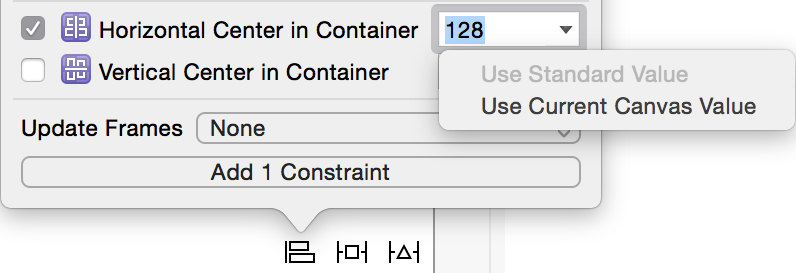
\includegraphics[width=200pt]{align_constraint_lesson_4.png}
	\end{center}
\end{figure}
\item Add another button, labeled "Magenta," to the bottom right of the interface, and add constraints similar to the previous Button.
\item Using Interface Builder and the Assistant Editor (\keys{\Alt+\cmd+\return}), establish connections between each button and two new controller methods, \texttt{changeBackgroundColorToWhite:} and \texttt{changeBackgroundColorToMagenta:}.
\begin{lstlisting}
@IBAction func changeBackgroundColorToWhite(sender: UIButton) {
}

@IBAction func changeBackgroundColorToMagenta(sender: UIButton) {
}
\end{lstlisting}
\item Implement the two methods.
\begin{lstlisting}
@IBAction func changeBackgroundColorToWhite(sender: UIButton) {
	view.backgroundColor = UIColor.whiteColor()
}

@IBAction func changeBackgroundColorToMagenta(sender: UIButton) {
	view.backgroundColor = UIColor.magentaColor()
}
\end{lstlisting}
\item Rename \texttt{changeBackgroundColor:} to \texttt{changeBackgroundColorToBlack:}, and observe that the adjacent connection well appears hollow.
\item Run the app (\keys{\cmd+R}), tap the Black button, and witness the app crash. Stop the app (\keys{\cmd+.}).
\item The app crashed because Interface Builder still tries to connect the button to the \texttt{changeBackgroundColor:} method, which no longer exists.
\item Using Interface Builder and the connection overlay, delete the old connection, establish a new connection to \texttt{changeBackgroundColorToBlack:}, and observe the connection well reappear.
\item Run the app (\keys{\cmd+R}), tap the buttons and witness the background color changing.
\end{itemize}

\end{document}
